\documentclass[]{article}
\usepackage{lmodern}
\usepackage{amssymb,amsmath}
\usepackage{ifxetex,ifluatex}
\usepackage{fixltx2e} % provides \textsubscript
\ifnum 0\ifxetex 1\fi\ifluatex 1\fi=0 % if pdftex
  \usepackage[T1]{fontenc}
  \usepackage[utf8]{inputenc}
\else % if luatex or xelatex
  \ifxetex
    \usepackage{mathspec}
  \else
    \usepackage{fontspec}
  \fi
  \defaultfontfeatures{Ligatures=TeX,Scale=MatchLowercase}
\fi
% use upquote if available, for straight quotes in verbatim environments
\IfFileExists{upquote.sty}{\usepackage{upquote}}{}
% use microtype if available
\IfFileExists{microtype.sty}{%
\usepackage{microtype}
\UseMicrotypeSet[protrusion]{basicmath} % disable protrusion for tt fonts
}{}
\usepackage[margin=1in]{geometry}
\usepackage{hyperref}
\hypersetup{unicode=true,
            pdftitle={Supporting Information for the manuscript: Bayesian non-asymptotic extreme value models for environmental data},
            pdfauthor={Enrico Zorzetto, Antonio Canale, and Marco Marani},
            pdfborder={0 0 0},
            breaklinks=true}
\urlstyle{same}  % don't use monospace font for urls
\usepackage{graphicx,grffile}
\makeatletter
\def\maxwidth{\ifdim\Gin@nat@width>\linewidth\linewidth\else\Gin@nat@width\fi}
\def\maxheight{\ifdim\Gin@nat@height>\textheight\textheight\else\Gin@nat@height\fi}
\makeatother
% Scale images if necessary, so that they will not overflow the page
% margins by default, and it is still possible to overwrite the defaults
% using explicit options in \includegraphics[width, height, ...]{}
\setkeys{Gin}{width=\maxwidth,height=\maxheight,keepaspectratio}
\IfFileExists{parskip.sty}{%
\usepackage{parskip}
}{% else
\setlength{\parindent}{0pt}
\setlength{\parskip}{6pt plus 2pt minus 1pt}
}
\setlength{\emergencystretch}{3em}  % prevent overfull lines
\providecommand{\tightlist}{%
  \setlength{\itemsep}{0pt}\setlength{\parskip}{0pt}}
\setcounter{secnumdepth}{0}
% Redefines (sub)paragraphs to behave more like sections
\ifx\paragraph\undefined\else
\let\oldparagraph\paragraph
\renewcommand{\paragraph}[1]{\oldparagraph{#1}\mbox{}}
\fi
\ifx\subparagraph\undefined\else
\let\oldsubparagraph\subparagraph
\renewcommand{\subparagraph}[1]{\oldsubparagraph{#1}\mbox{}}
\fi

%%% Use protect on footnotes to avoid problems with footnotes in titles
\let\rmarkdownfootnote\footnote%
\def\footnote{\protect\rmarkdownfootnote}

%%% Change title format to be more compact
\usepackage{titling}

% Create subtitle command for use in maketitle
\providecommand{\subtitle}[1]{
  \posttitle{
    \begin{center}\large#1\end{center}
    }
}

\setlength{\droptitle}{-2em}

  \title{Supporting Information for the manuscript: Bayesian non-asymptotic
extreme value models for environmental data}
    \pretitle{\vspace{\droptitle}\centering\huge}
  \posttitle{\par}
    \author{Enrico Zorzetto, Antonio Canale, and Marco Marani}
    \preauthor{\centering\large\emph}
  \postauthor{\par}
      \predate{\centering\large\emph}
  \postdate{\par}
    \date{4/30/2020}

\usepackage{multirow}

\begin{document}
\maketitle

\renewcommand{\thefigure}{S\arabic{figure}}
 \renewcommand{\thetable}{S\arabic{table}}
 \renewcommand{\theequation}{S\arabic{equation}}

\hypertarget{details-on-the-bayesian-gev-and-pot-models-implemented}{%
\section{Details on the Bayesian GEV and POT models
implemented}\label{details-on-the-bayesian-gev-and-pot-models-implemented}}

Here we breafly review the main extreme value statistical models
consistently with the notation used in this manuscript. The two
approaches detailed below are the Generalized Extreme Value distribution
used as a model for block maxima series, and the Peak Over Threshold
(POT) defined as a Poisson point process. For a complete discussion, see
Coles (2001) or De Haan and Ferreira (2007). These models are commonly
used for EV analysis and statistical software that implement these
technique is available, such as for example the \emph{extRemes} R
package (Gilleland, Katz, and others 2016). The Bayesian estimation for
the GEV and POT models used in our study is described below and
implemented in the HMEV R package.

\hypertarget{the-generalized-extreme-value-distribution}{%
\subsection{The Generalized Extreme Value
distribution}\label{the-generalized-extreme-value-distribution}}

The (GEV) distribution (Von Mises 1936) has cdf \begin{equation}
    Pr \left(Y \le y\right) =  F_{GEV} \left(y \mid \mu, \sigma, \xi \right) = \exp \left\{ -\left( 1 + \frac{\xi}{\sigma}\left( y - \mu \right)
    \right)_{+}^{-1/\xi} \right\}.
    \label{eq:gev}
\end{equation} where \(\mu \in R\) and \(\sigma \in R^{+}\) are location
and scale parameters respectively, while \(\xi \in R\) is a shape
parameter, and \((\cdot)_{+} = \max\left\{ 0, \cdot \right\}\).
Depending on the value of \(\xi\), the GEV family encompasses a double
exponential, an heavy-tailed, and an upper bounded distribution.

The GEV parameters are generally estimated by means of Maximum
Likelihood (ML), Penalized ML (Martins and Stedinger 2000), L-Moments
(Hosking 1990) or Bayesian methods (S. G. Coles and Tawn 1996,
@coles2003fully). Confidence intervals can be obtained with the Delta
method in the case of ML inference (Coles 2001) or using Bootstrap
techniques when the L-moments are used to fit the distribution.
Generally L-moments perform better than ML in the case of small samples,
even though asyntotic theory for confidence intervals is not available.
Bayesian Methods allow better characterization of the variability of
extimated values (S. G. Coles and Tawn 1996; S. G. Coles and Powell
1996; Coles, Pericchi, and Sisson 2003; Stephenson and Tawn 2004). Here
we use Bayesian methods for fitting the GEV model (we implemented a Stan
model, sampling from the posterior using the Hamiltonian Monte Carlo
sampler as done for HMEV). This gives us Bayesian probability intervals
for the GEV quantiles for a given return time. We elicit the prior
distributions for the three GEV parameters as follows: For the shape
parameter, we select as prior distribution a normal distribution
centered in 0.114 with a standard deviation \(\sigma = 0.125\). This
choice matches the expected value suggested globally by (Koutsoyiannis
2004), while the overall shape of the Prior distribution closely match
the Geophysical Prior proposed by (Martins and Stedinger 2000) in order
to guide inference towards reaslistc values of the shape parameter. For
the shape and scale parameters, we select informative prior centered
around the mean and standard deviation of the annual maxima samples, in
order to exploit prior knoiwledge on the expected value and
characteristic variability of annual maxima values.

\hypertarget{the-peak-over-threshold-method}{%
\subsection{The Peak Over Threshold
method}\label{the-peak-over-threshold-method}}

The GEV distribution also arises as limiting model for the block maxima
of a point process with Poisson-distributed arrival of events with
magnitudes distributed according to a Generalized Pareto distribution,
which is often used to model exceedance over a high threshold (Davison
and Smith 1990). The distribution of exceedances over a high threshold
\(q\) is

\begin{equation}
    Pr \left( Y > y\right) = Pr \left( X > x + q \lvert X > q\right) \simeq
    \frac{1 - F(x + q)}{1 - F(u)} = 1 - F_{GPD} \left( x \lvert q, \beta,
    \kappa \right)
    = \left(
    1 + \frac{\kappa}{\beta}\left( x - \mu \right)\right)^{-1/\kappa}
\end{equation}

In this case, the distribution of block maxima reads

\begin{equation}
    F_{PP} \left(x \right) = \sum_{n = o}^{\infty}p_n(n \lvert \lambda)F_{GPD} \left(x \lvert
    \beta, q, \kappa \right)
    =1 - \sum_{n = o}^{\infty} \frac{\lambda^n e^{-\lambda}}{n!}\left(
    1 + \frac{\kappa}{\beta}\left( x - q\right)\right)^{-1/\kappa}
    = F_{GEV} \left( x \lvert \mu, \sigma, \xi \right)
\end{equation}

where the parameters of the GEV are obtained as follows
\(\kappa = \xi\), \(\beta = \sigma +\xi \left( q - \mu \right)\), and
\(\lambda = \left( 1 + \xi \frac{\xi}{\beta}\left( q - \mu \right)\right)^{-1/\xi}\)

Here we use Bayesian inference for this Poisson-GPD model for threshold
exceedances. We elicit the prior distribution for the model parameters
as follows: For the Pareto shape parameter, we choose the same
informative prior elicited for the GEV - annual maxima model. For the
Poisson rate, we select a prior distribution centered on \(4\)
events/year, which appears reasonable value since we fix the threshold
based on a fixed number of average exceedances in each block. For our
analysis, we choose an automated threshold such that \(5\%\) of the
non-zero values are above threshold.

Once we draw from the posterior samples for these parameters
\(\lambda^{(s)}\), \(\beta^{(s)}\), and \(\kappa^{(s)}\), for
\(s = 1, \dots, S\), we can compute the posterior probability for the
quivalent parameters of the GEV model as follows:

\(\mu^{(s)} = q + \frac{\beta^{(s)}}{\kappa^{(s)}} \left( \lambda^{(s) ^{\kappa^{(s)}}} - 1\right)\)
\(\sigma^{(s)} = \beta^{(s)} \lambda^{(s) ^{\kappa^{(s)}}}\)
\(\xi^{(s)} = \kappa^{(s)}\)

\hypertarget{definitions-of-lppd-and-lpml}{%
\subsection{Definitions of lppd and
lpml}\label{definitions-of-lppd-and-lpml}}

Evaluating the predictive accuracy of extreme value models in estimating
the right tail of the distribution is indeed an inherently challenging
task, as high quantiles are, by definition, poorly represented in the
available samples. For this reason, cross validation techniques are
rarely used to assess the performance of fitted extreme value models. In
our analysis, however, we harnessed the considerable length of the
synthetic data sets available here in order to extensively test the
performance of different methods using both in-sample and out-of-sample
validation techniques. To this end, we employ both in-sample and
out-of-sample measures.

The log pointwise predictive density (lppd) (Gelman et al. 2013)
computed both for the in-sample data and for the out-of-sample data is
often used as a measure of global performance of the models.

This can be directly estimated from \(S\) draws from a MCMC sameple as

\begin{equation}
        \widehat{lppd} = \sum_{i = 1}^{n} \log \left( \frac{1}{S}\sum_{s = 1}^{S} p(y_i \lvert
    {\theta}^{(s)})\right)
\end{equation} This quantity, if computed for in-sample data \(y_i\), is
expected to overestimate the expected log predictive density (elpd) for
the same data points. This overestimation is generally corrected by
quantifying the overfit of the model using some estimate of the
effective number of parameter of the model. Common corrections used in
practice include the Deviance Information Crtiterion (DIC),
Watanaibe-Aikake information criterion (WAIC) (Gelman et al. 2013), or
leave one out techniques such as the log posterior marginal likelihood
(LPML) (Gelfand and Dey 1994), or leave-one-out based on Pareto Smoothed
Importance Sampling (PSIS) , (Vehtari, Gelman, and Gabry 2017).

Here we used the logarithm of the pseudo-marginal likelihood (lpml), a
convenient index that directly accounts, at no additional computational
cost, for a leave-one-out cross validation measure (Gelfand and Dey
1994). Notably, since the lpml approximates the expected log pointwise
predictive density, the difference between the in-sample lppd and the
lpml represents the number of effective parameters of a model (Vehtari,
Gelman, and Gabry 2017) and thus will be used to quantify overfitting.

\begin{equation}
    lpml_m = -\frac{1}{m}\sum_{i = 1}^{m} \log{\left( CPO_i \right)}
\end{equation}

where we add the factor \(-1/m\) to reduce its variation with sample
size. Here \(CPO_i\) is the \emph{Conditional Predictive Ordinate}
statistics introduced by (Gelfand, Dey, and Chang 1992) and (Gelfand and
Dey 1994), which estimates the probability of observing a value \(y_i\)
given that \(\mathbf{y}_{-i}\) has been observed. \(CPO_i\) can be
obtained as follows:

\begin{equation}
    CPO_i =  \left\{\int \frac{1}{p\left( y_i \mid
        \mathbf{\theta}\right)} p \left( \mathbf{\theta} \mid
    \mathbf{y_{-1}} \right) d \mathbf{\theta} \right\}^{-1}
\end{equation}

The CPO can be computed as the geometric mean of the likelihood of the
data (annual maxima) given the model. Sampling from the posterior, one
can compute\(CPO_i\) as follows:

\begin{equation}
    \widehat{CPO_i} = \left[ \frac{1}{S} \sum_{s = 1}^{S} \frac{1}{p\left( y_i \mid
    \mathbf{\theta}^{\left(s\right)}\right)}\right]^{-1}
\end{equation}

Therefore \(CPO_i\) can be computed as the harmonic mean of the
likelihood of the annual maxima \(y_i\) given the model. The best model
amongst the ones tested here will be characterized by the largest value
of \(LPML\). Note that given the properties of this measure of
predictive performance (in essence equivalent to a leave-one-out cross
validation), we can use LPML when a single sample is available for
calibration and testing of the EV models. Therefore, LPML can be used to
decide which of these models is best for a given sample/ application. We
therefore propose to use it when only short samples are available to
decide which EV model we shouls use for the distribution of annual
maxima. We note that LPML can be difficult to use for the GEV
distribution when applied to a validation sample different from the one
used to fit the distribution, since it is possible that the modelled
posterior distribution assign zero probability to some of the observed
values.

\section{Additional tables}

\begin{table}[h]
    \centering
    \caption{Summary of 4 model specifications used to generate synthetic datasets in the simulation study.}
    \begin{tabular}{ll}

        \hline
        Model for $x_{ij}$  & parameters \\ \hline

        GP  & $\xi = 0.1, \quad \sigma = 8$ \\
        GAM  & $\alpha = 1.2, \quad \beta = 0.12$ \\
        WEI  & $\gamma = 0.6, \quad \delta = 8 $ \\
        WEI$_G$  & $\mu_{\delta} = 7, \quad \sigma_{\delta} = 1, \quad \mu_{\gamma} = 1, \quad \sigma_{\gamma} = 0.1,$ \\
        \hline
        Model for $n_{j}$  & parameters \\ \hline
        BBN & $ \mu_n = 100, \quad \sigma^2_n = 150 $  \\ \hline

        \label{tab:simulations}
    \end{tabular}
\end{table}

\begin{table}
    \centering
    \caption{Values of the constants used to elicit the prior hyperparameters of the model for event magnitudes.}
    \begin{tabular}{ llll }
        % \begin{tabular}{ lccc }
        \hline
        Parameter  & Value  \\ \hline
        \hline
        $\alpha_{\mu \gamma 0}=$   &  $i_{\mu \gamma 0} $ \\
        $\beta_{\mu \gamma 0}=$   &  $i_{\mu \gamma 0} \cdot e_{\mu \gamma 0} $ \\

        $\alpha_{\mu \delta 0}=$   &  $i_{\mu \delta 0} $ \\
        $\beta_{\mu \delta 0}=$   &  $i_{\mu \delta 0} \cdot e_{\mu \delta 0} $ \\

        $\alpha_{\sigma \gamma 0}=$   &  $i_{\sigma \gamma 0} $ \\
        $\beta_{\sigma \gamma 0}=$   &  $i_{\sigma \gamma 0} \cdot e_{\sigma \gamma 0} \cdot v_{\sigma \gamma 0} $ \\

        $\alpha_{\sigma \delta 0}=$   &  $i_{\sigma \delta 0} $ \\
        $\beta_{\sigma \delta 0}=$   &  $i_{\sigma \delta 0} \cdot e_{\sigma \delta 0} \cdot  v_{\sigma \delta 0} $ \\


        \hline
        Constant  & Value & Meaning & Empirical Prior \\ \hline

        $i_{\mu \gamma 0}$  & 10 & shape informativeness  & no \\
        $i_{\mu \delta 0}$  & 10 & scale informativeness & no \\

        $i_{\sigma \gamma 0}$  & 10 & shape informativeness & no \\
        $i_{\sigma \delta 0}$  & 10 & scale informativeness & no \\

        $e_{\mu \gamma 0}$  & 0.7 & expected value shape & no \\
        $e_{\mu \delta 0}$  & $10/ \Gamma \left( 1 + 1/{0.7}\right)$ & expected value scale &  no (possible)\\

        $v_{\sigma \gamma 0}$  & 0.05 & expected variability shape & no \\
        $v_{\sigma \delta 0}$  & 0.25 & expected variability scale &  no (possible) \\



        \hline



        \label{tab:priors}
    \end{tabular}
\end{table}

\%

\begin{table}
    \centering
    \caption{Summary of the model for the number of arrivals.}
    \begin{tabular}{ lccc }
        % \begin{tabular}{ lccc }
        \hline
        Model  & Outer level & Inner Level & Prior \\ \hline
        \multirow{1}{*}{ Binomial }


        & $n_j \sim Bin(\pi_0)$ &  & $\pi_0 \sim Beta\left( 2, 2\right)$
        \\
        \hline

        \multirow{3}{*}{ Beta Binomial }  & $n_j \sim Bin(\pi_0)$ & $\pi_0 \sim Beta\left( \alpha_n, \beta_n\right)$   & $\mu_n ~ \Gamma \left( 10, 0.1 \right)$
        \\
        & & & $\omega_n ~ \Gamma \left( 0.2, 0.2 \right)$
        \\
        & &    & $ \alpha_n = \left( 1 - \frac{\left(\omega_n + 1 \right)}{ \left( N_t - \mu_n \right) } \right) / \left(   \frac{\left(\omega_n + 1 \right)}{ \left( N_t - \mu_n \right) } N_t - 1\right) $
        \\

        & &    & $ \beta_n = \frac{\alpha_n}{\mu_n} \left( N_t - \mu_n\right)$
        \\

        \hline


        \label{tab:nmodels}
    \end{tabular}
\end{table}

\hypertarget{stations-effective-number-of-parameters}{%
\subsection{Stations: Effective number of
parameters}\label{stations-effective-number-of-parameters}}

As we can see in Figure \ref{fig:effnumpar} we report the effective
number of paramaters computed for observed data. Additionally, we
include the same quantity computed in a different way (Watanabe-Aikake
information criterion) to show that results do not change too much.

\begin{figure}
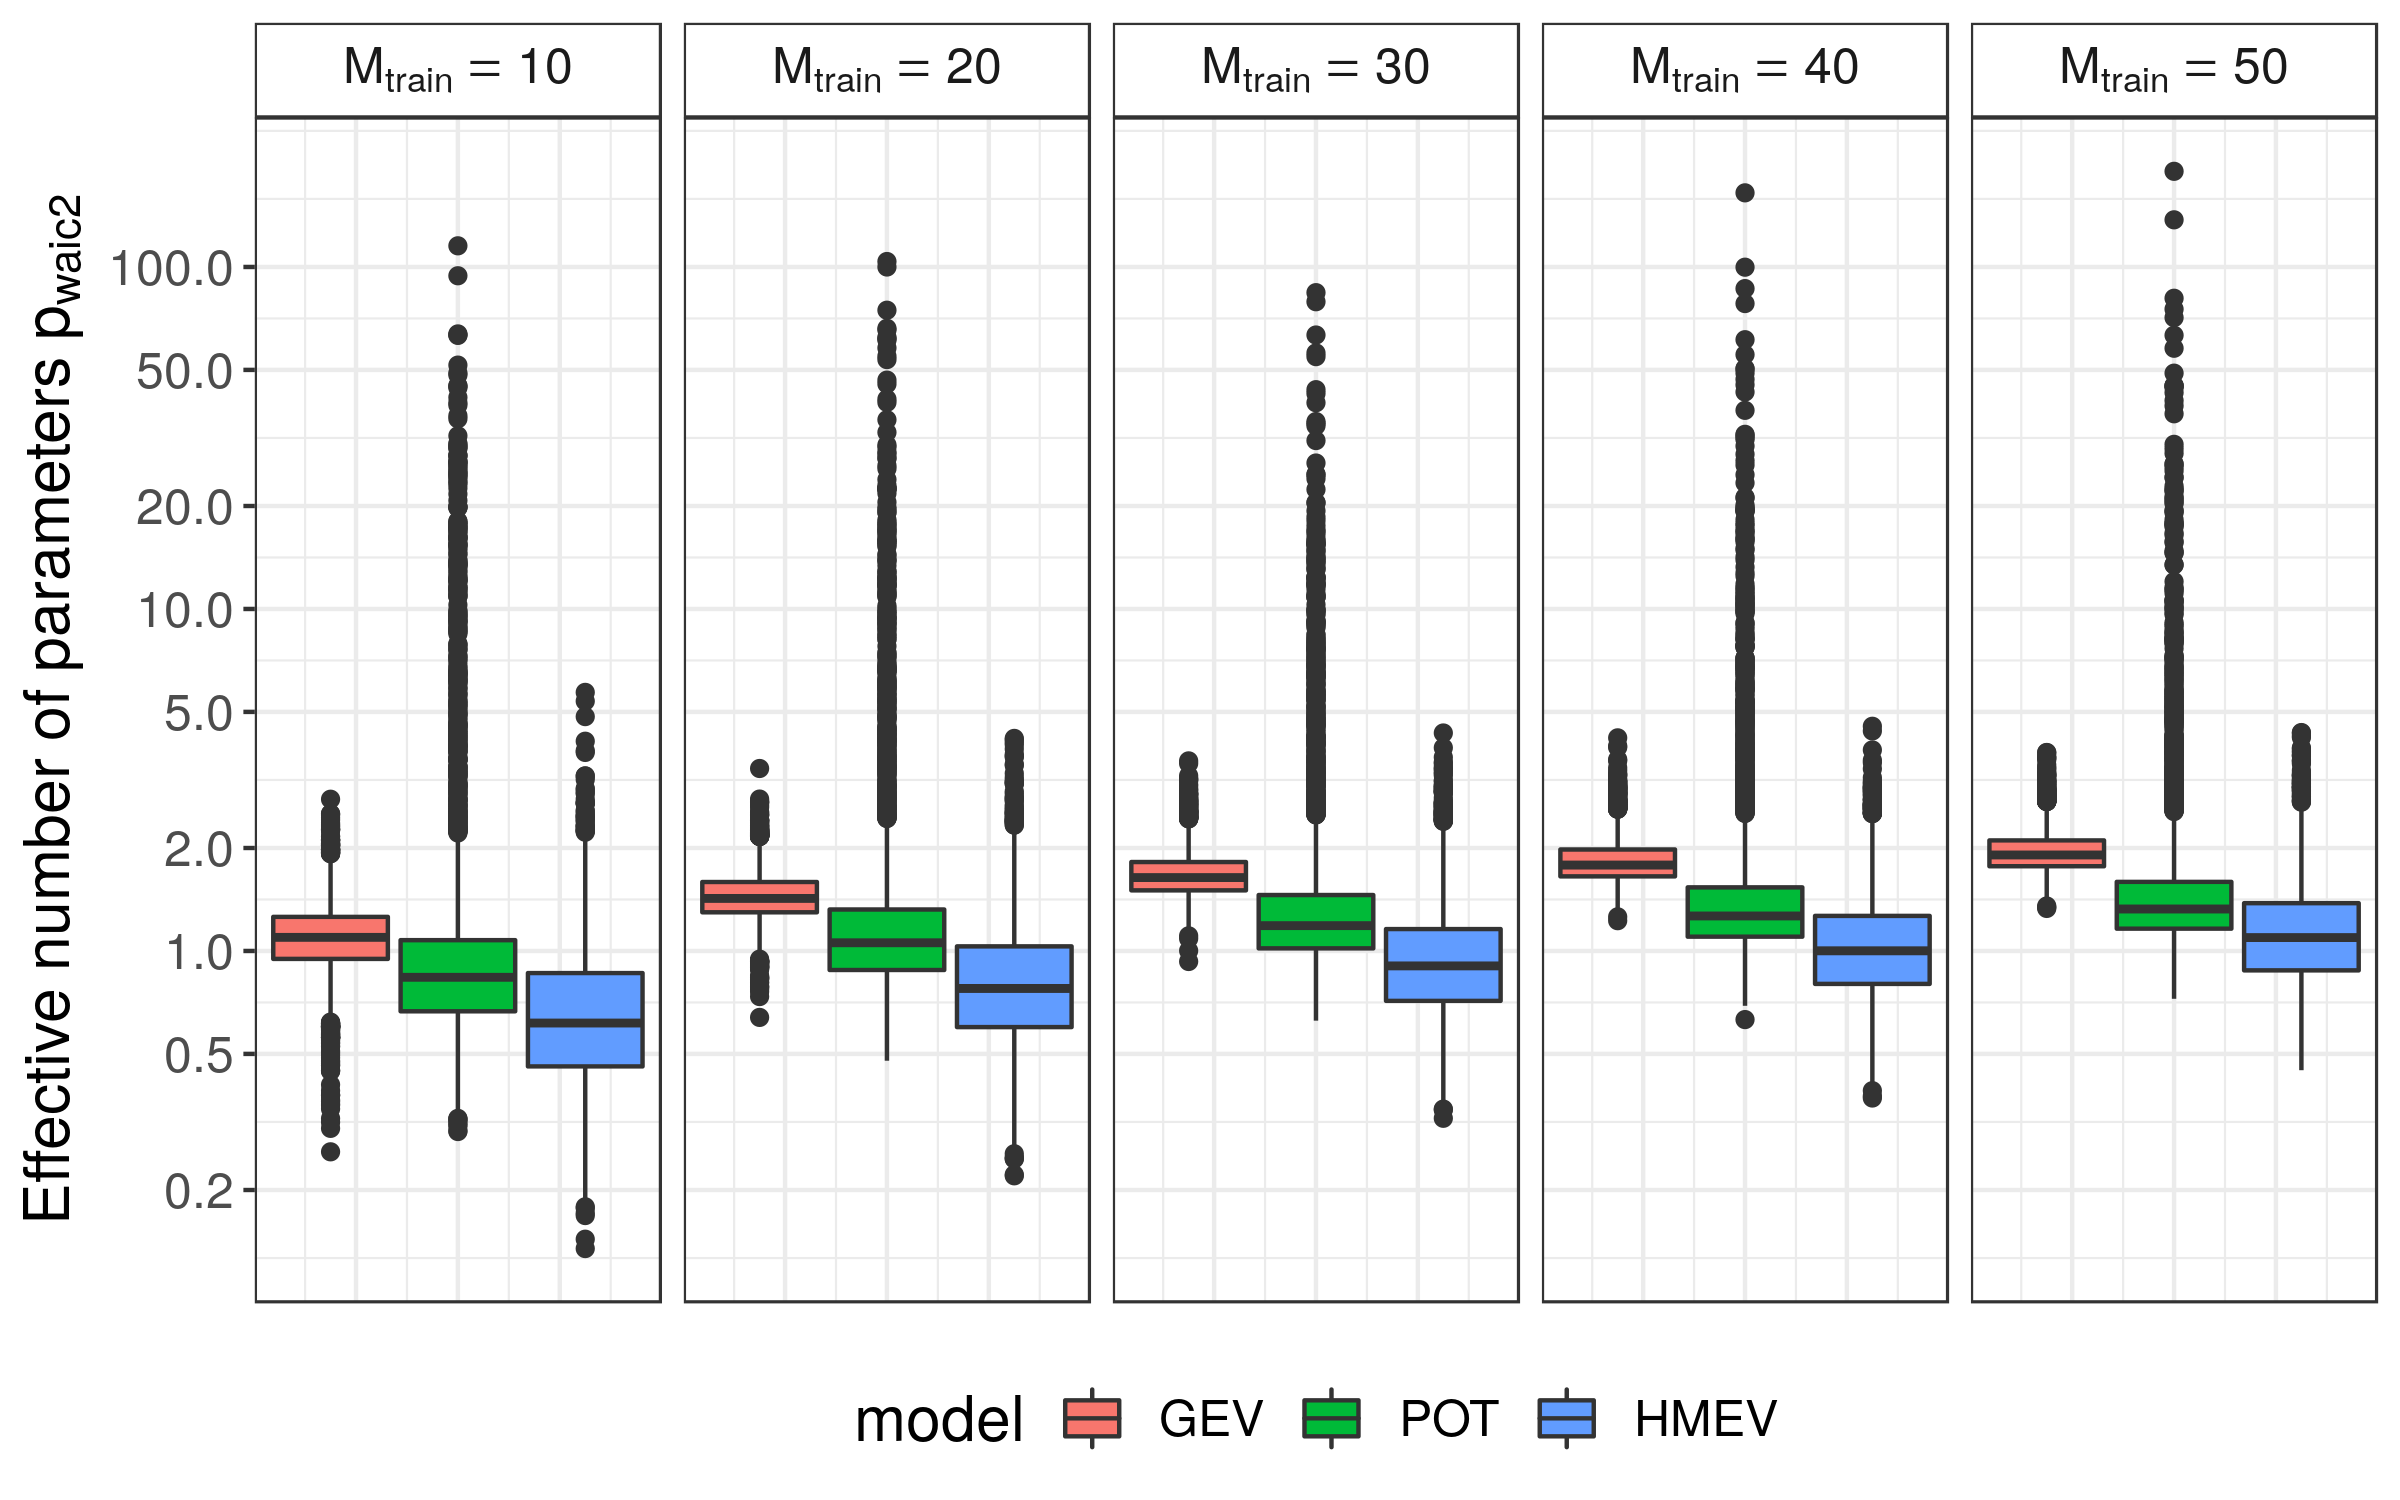
\includegraphics[width=1\linewidth]{../output/outplot/eff_num_par_waic2_kfold_479_0_dec} \caption{Effective number of parameters for the stations in the USHCN dataset.\label{fig:effnumpar}}\label{fig:effnumpar}
\end{figure}

\hypertarget{spatial-distribution-of-the-results-for-lppd-and-fse}{%
\subsection{Spatial distribution of the results for LPPD and
FSE}\label{spatial-distribution-of-the-results-for-lppd-and-fse}}

As we can see in Figure \ref{fig:maps_lppd}, here are the results for
the three models evaluated using the LPPD

Here we provide a spatially-explicit representation of model
performances, by mapping, in Figures \ref{fig:maps_lppd} and
\ref{fig:maps_fse}, the best model for each station as evaluated through
the lppd pr FSE measures respectively. This representation of the
results of our analysis shows again the interesting difference observed
for the in-sample analysis, which tend to favor the POT method, and the
out-of-sample results where HMEV appears to be selected most often as
preferred model. The frequency of HMEV being the model of choice is
higher for smaller sample sizes.

\begin{figure}
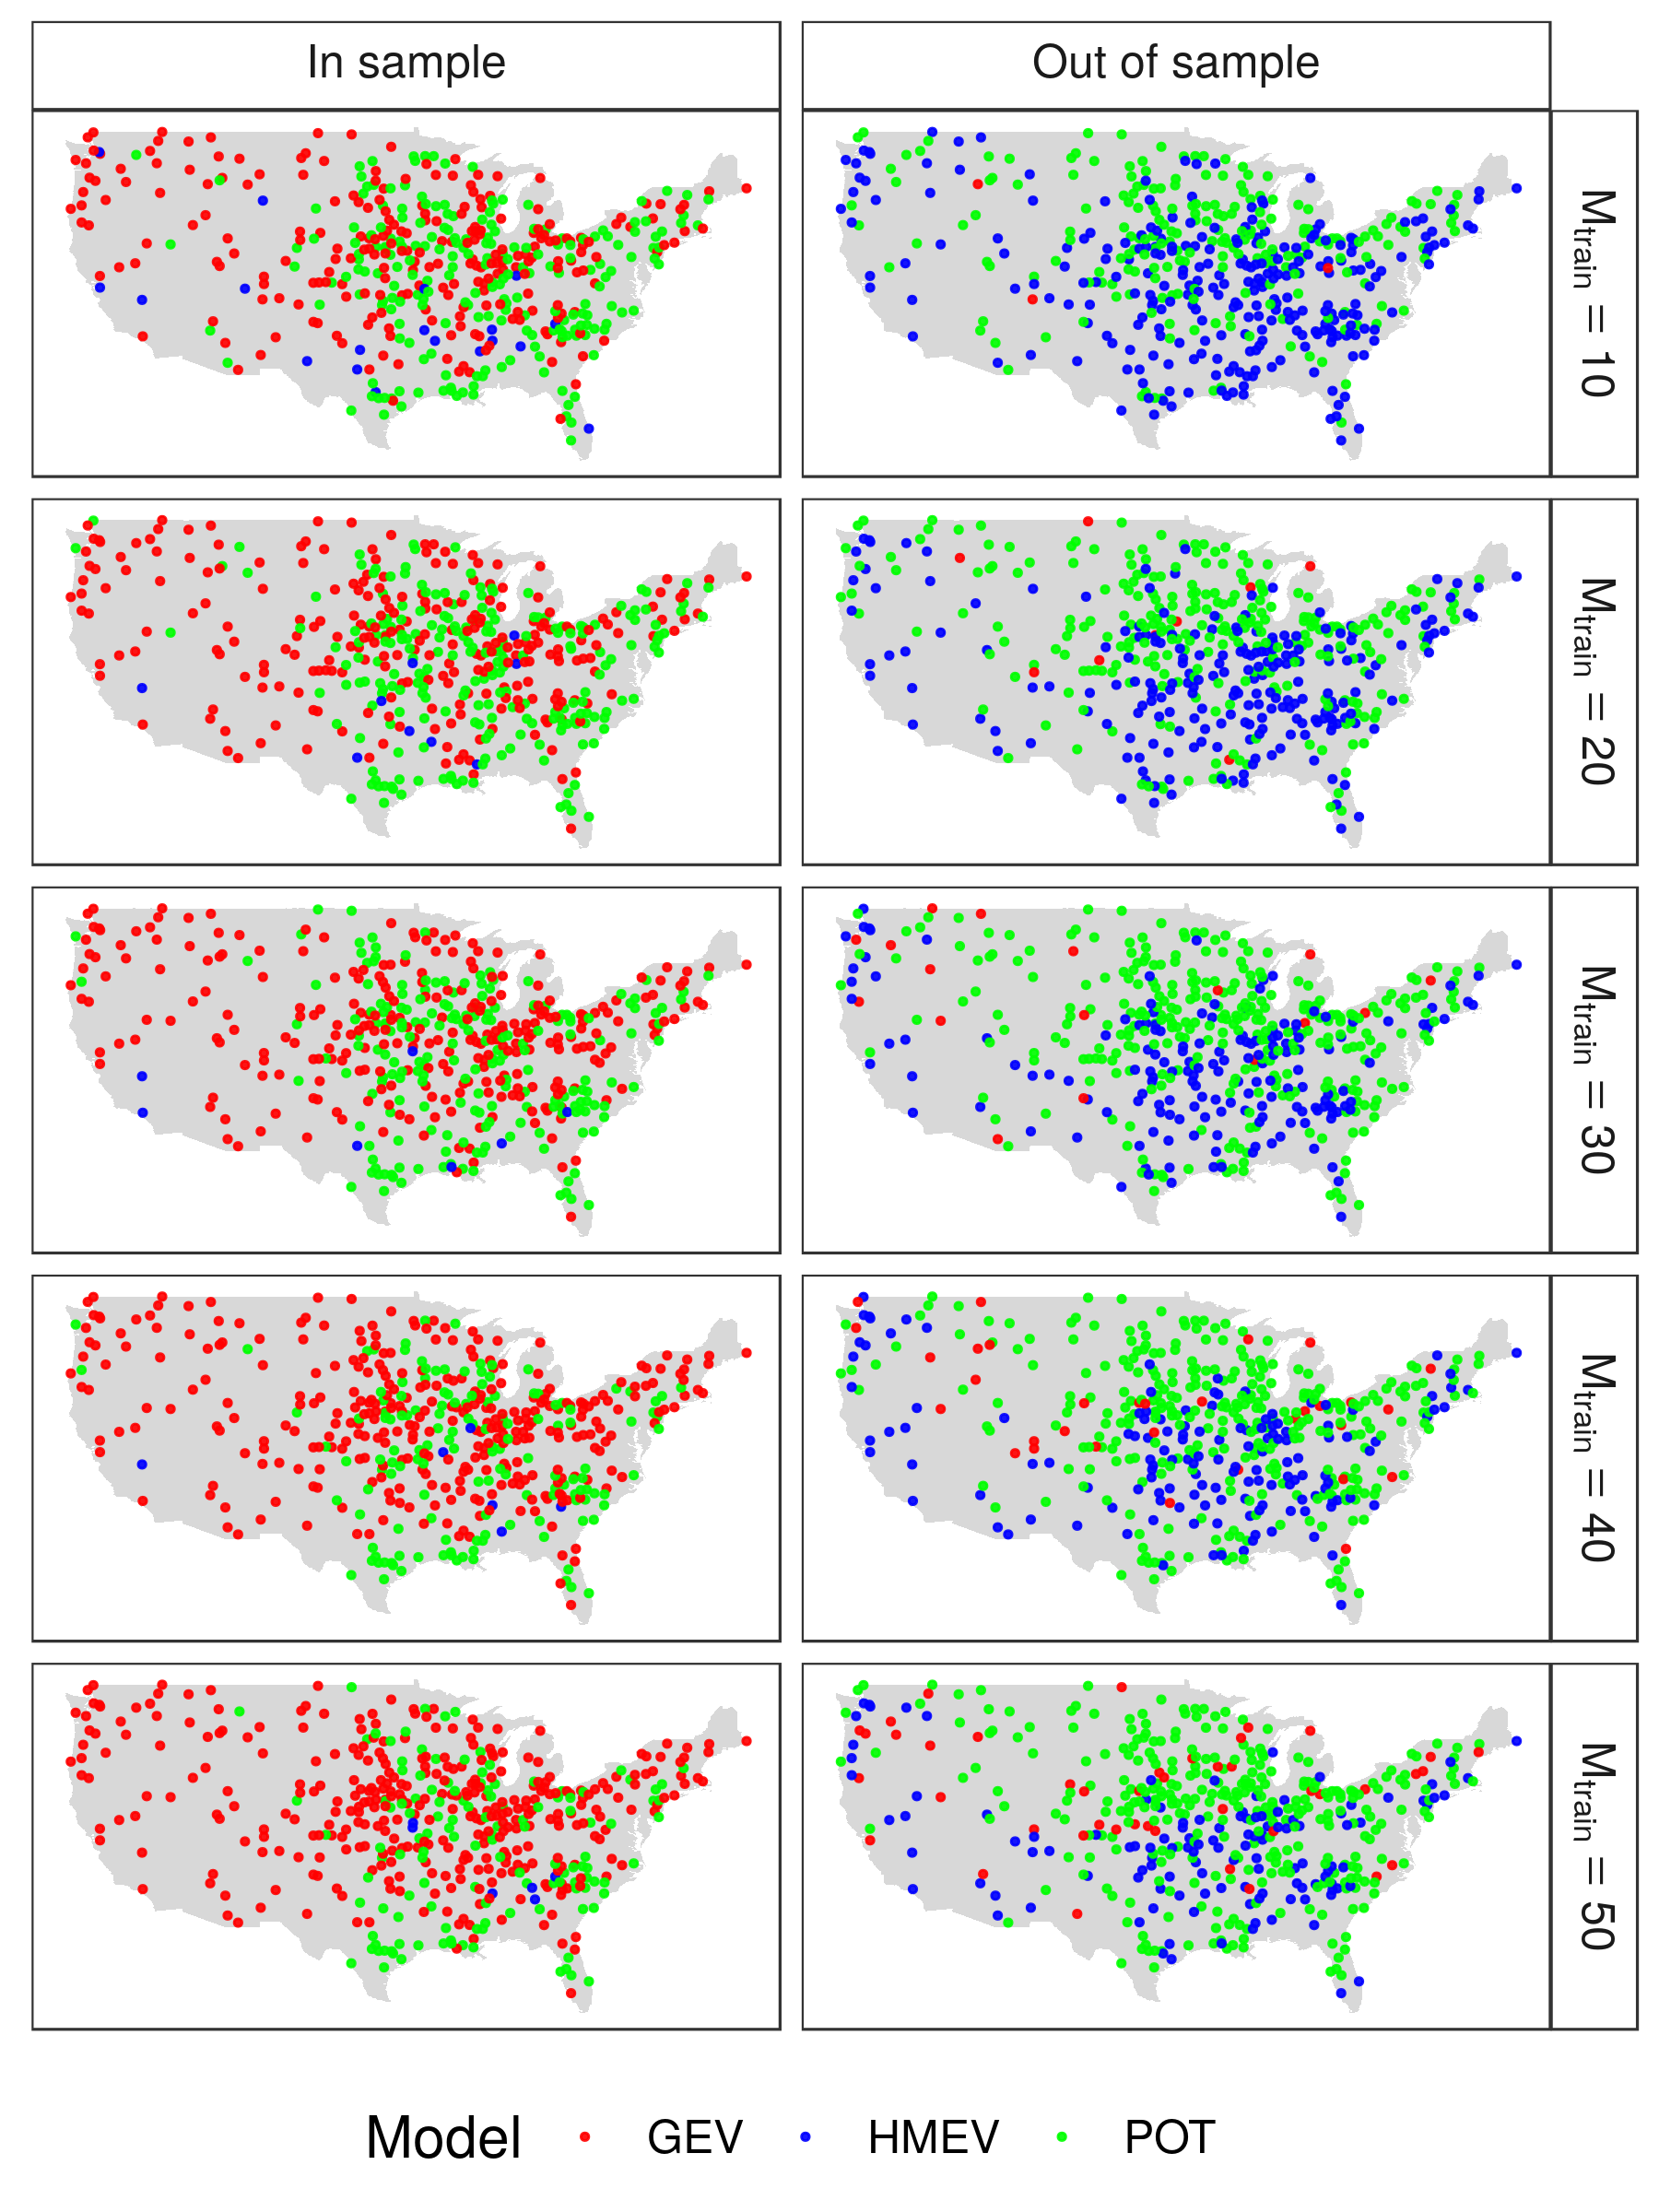
\includegraphics[width=1\linewidth]{../output/outplot/lppd_maps_kfold_479_0_dec} \caption{Best model for each station, as evaluated through the LPPD measure (in-sample and out-of-sample).\label{fig:maps_lppd}}\label{fig:maps1}
\end{figure}

And in Figure \ref{fig:maps_fse} we report the same result for the FSE

\begin{figure}
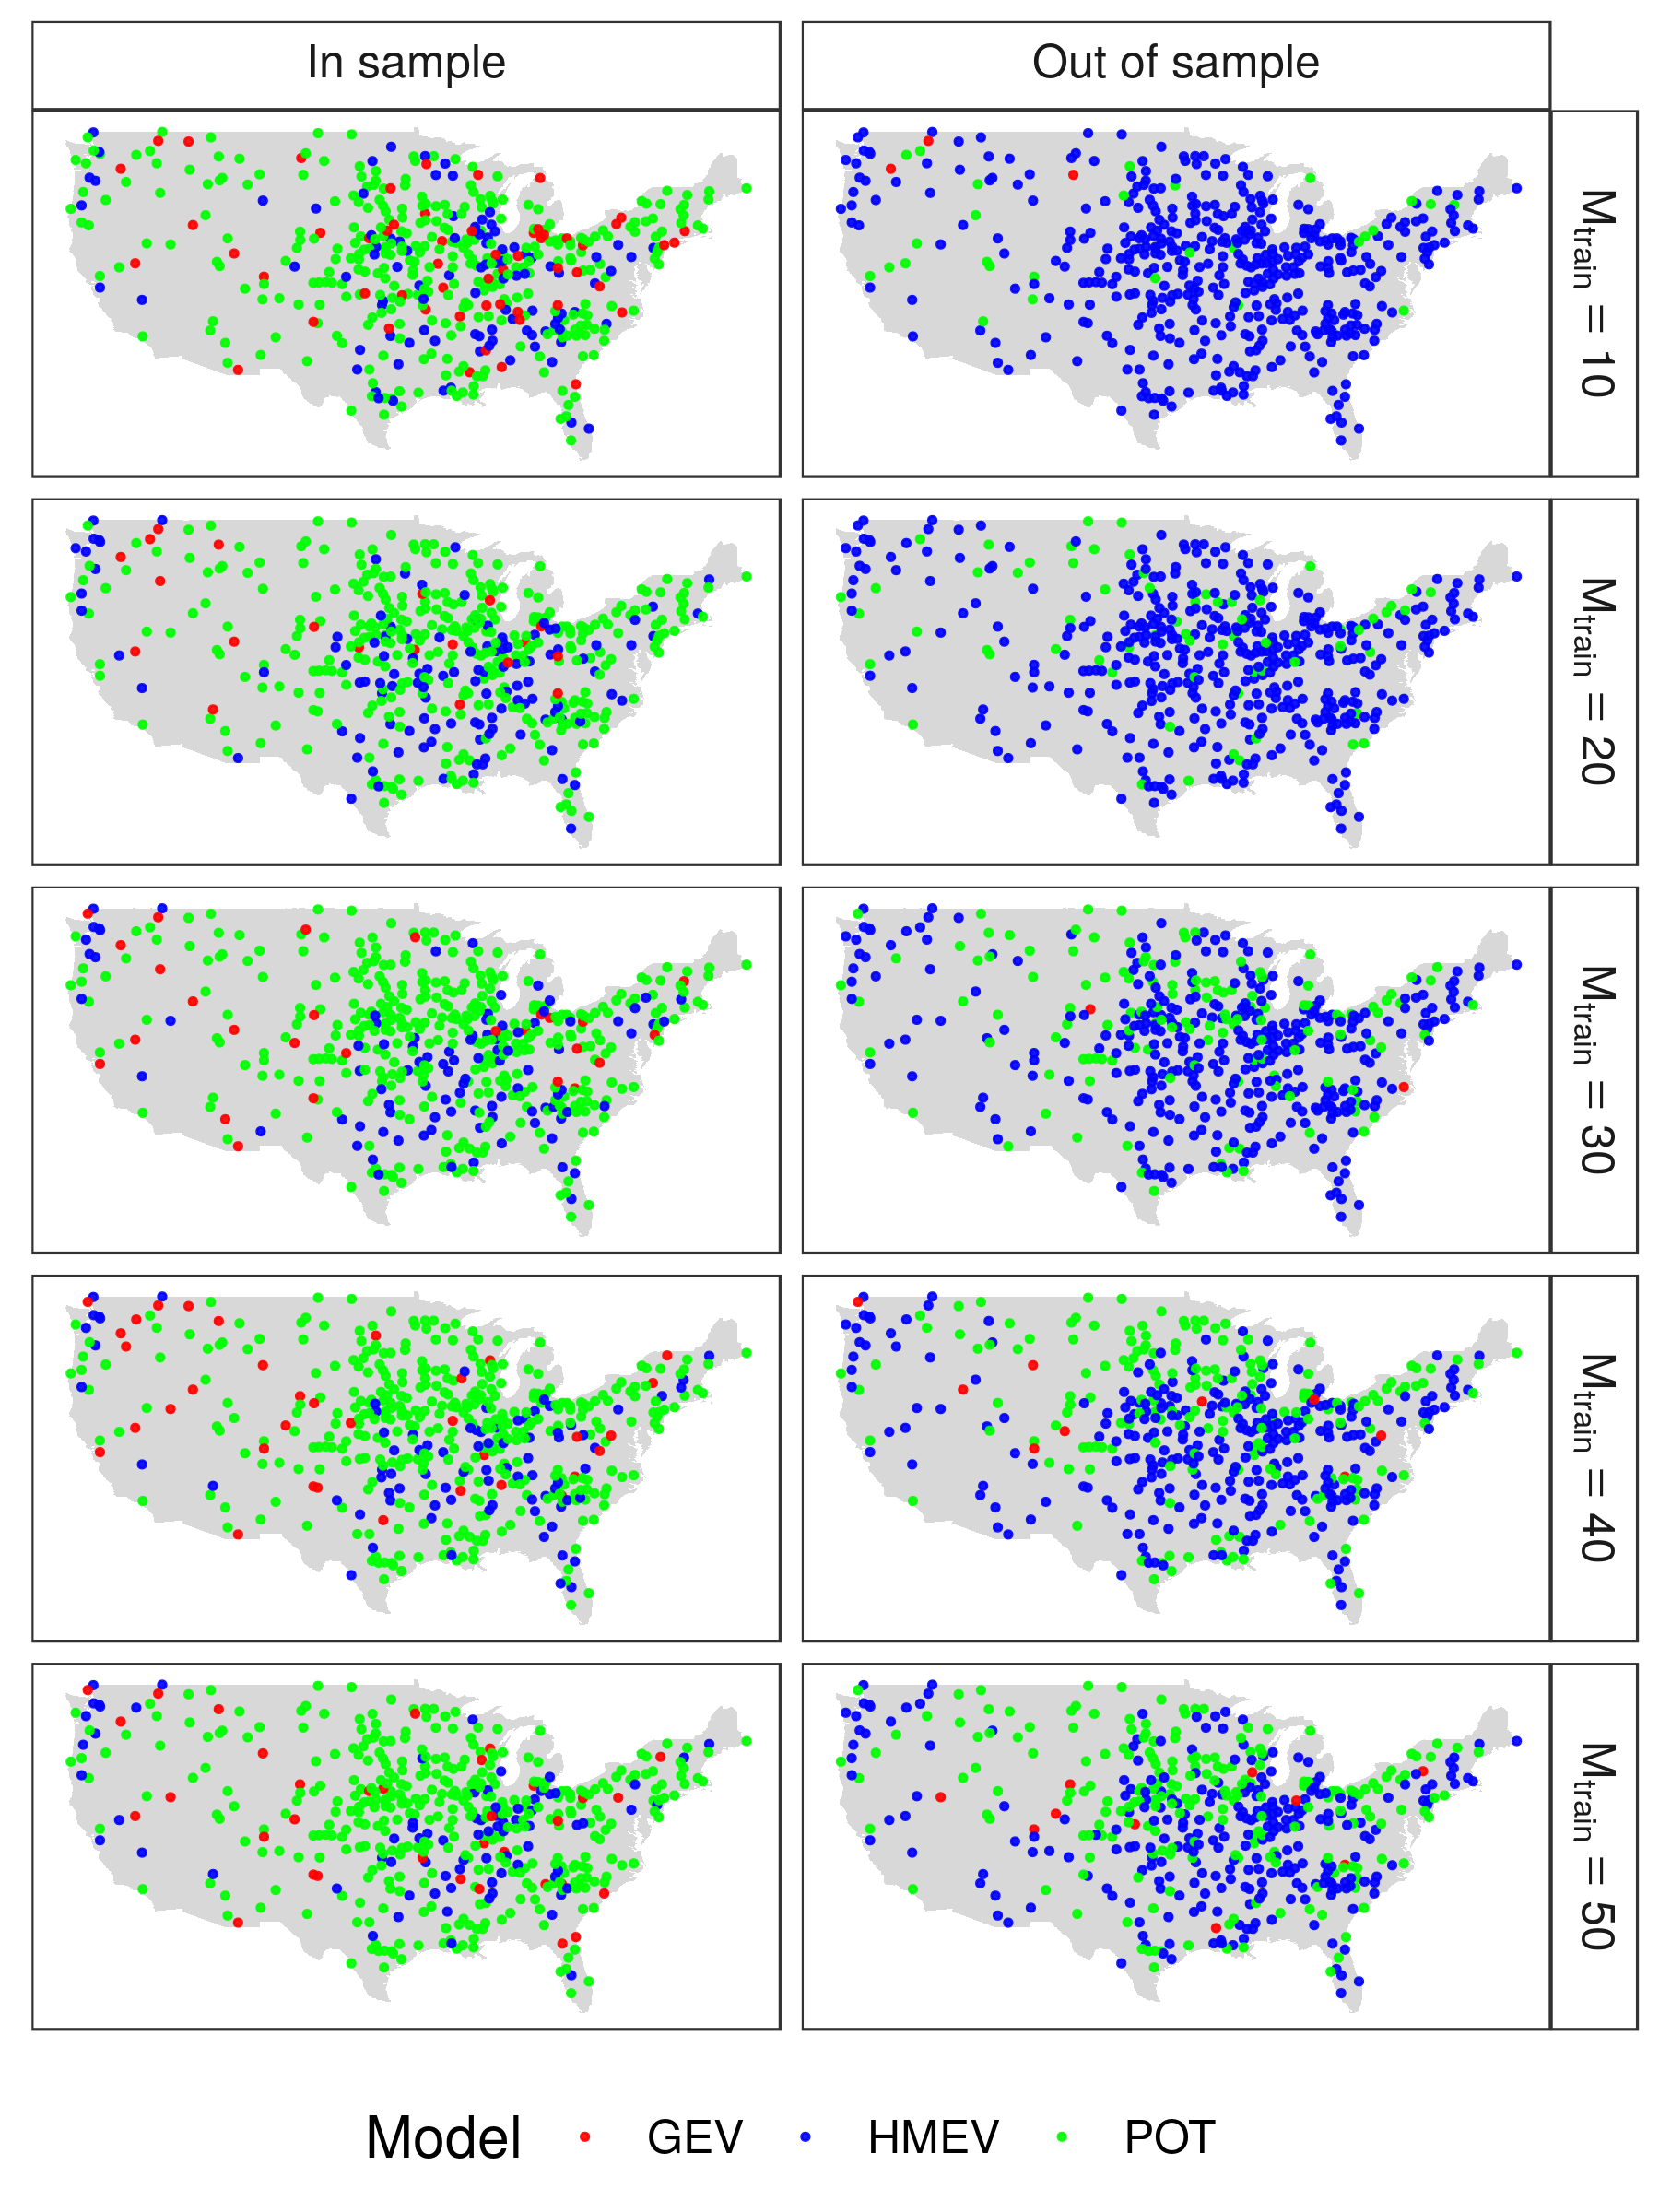
\includegraphics[width=1\linewidth]{../output/outplot/fse_maps_kfold_479_0_dec} \caption{Best model for each station, as evaluated through the FSE measure (in-sample and out-of-sample).\label{fig:maps_fse}}\label{fig:maps2}
\end{figure}

in Figures \ref{fig:wei_spec}, \ref{fig:gam_spec}, and
\ref{fig:gpd_spec} we report examples using the Weibull, Gamma, and
Generalized Pareto specifications respectively.

\begin{figure}
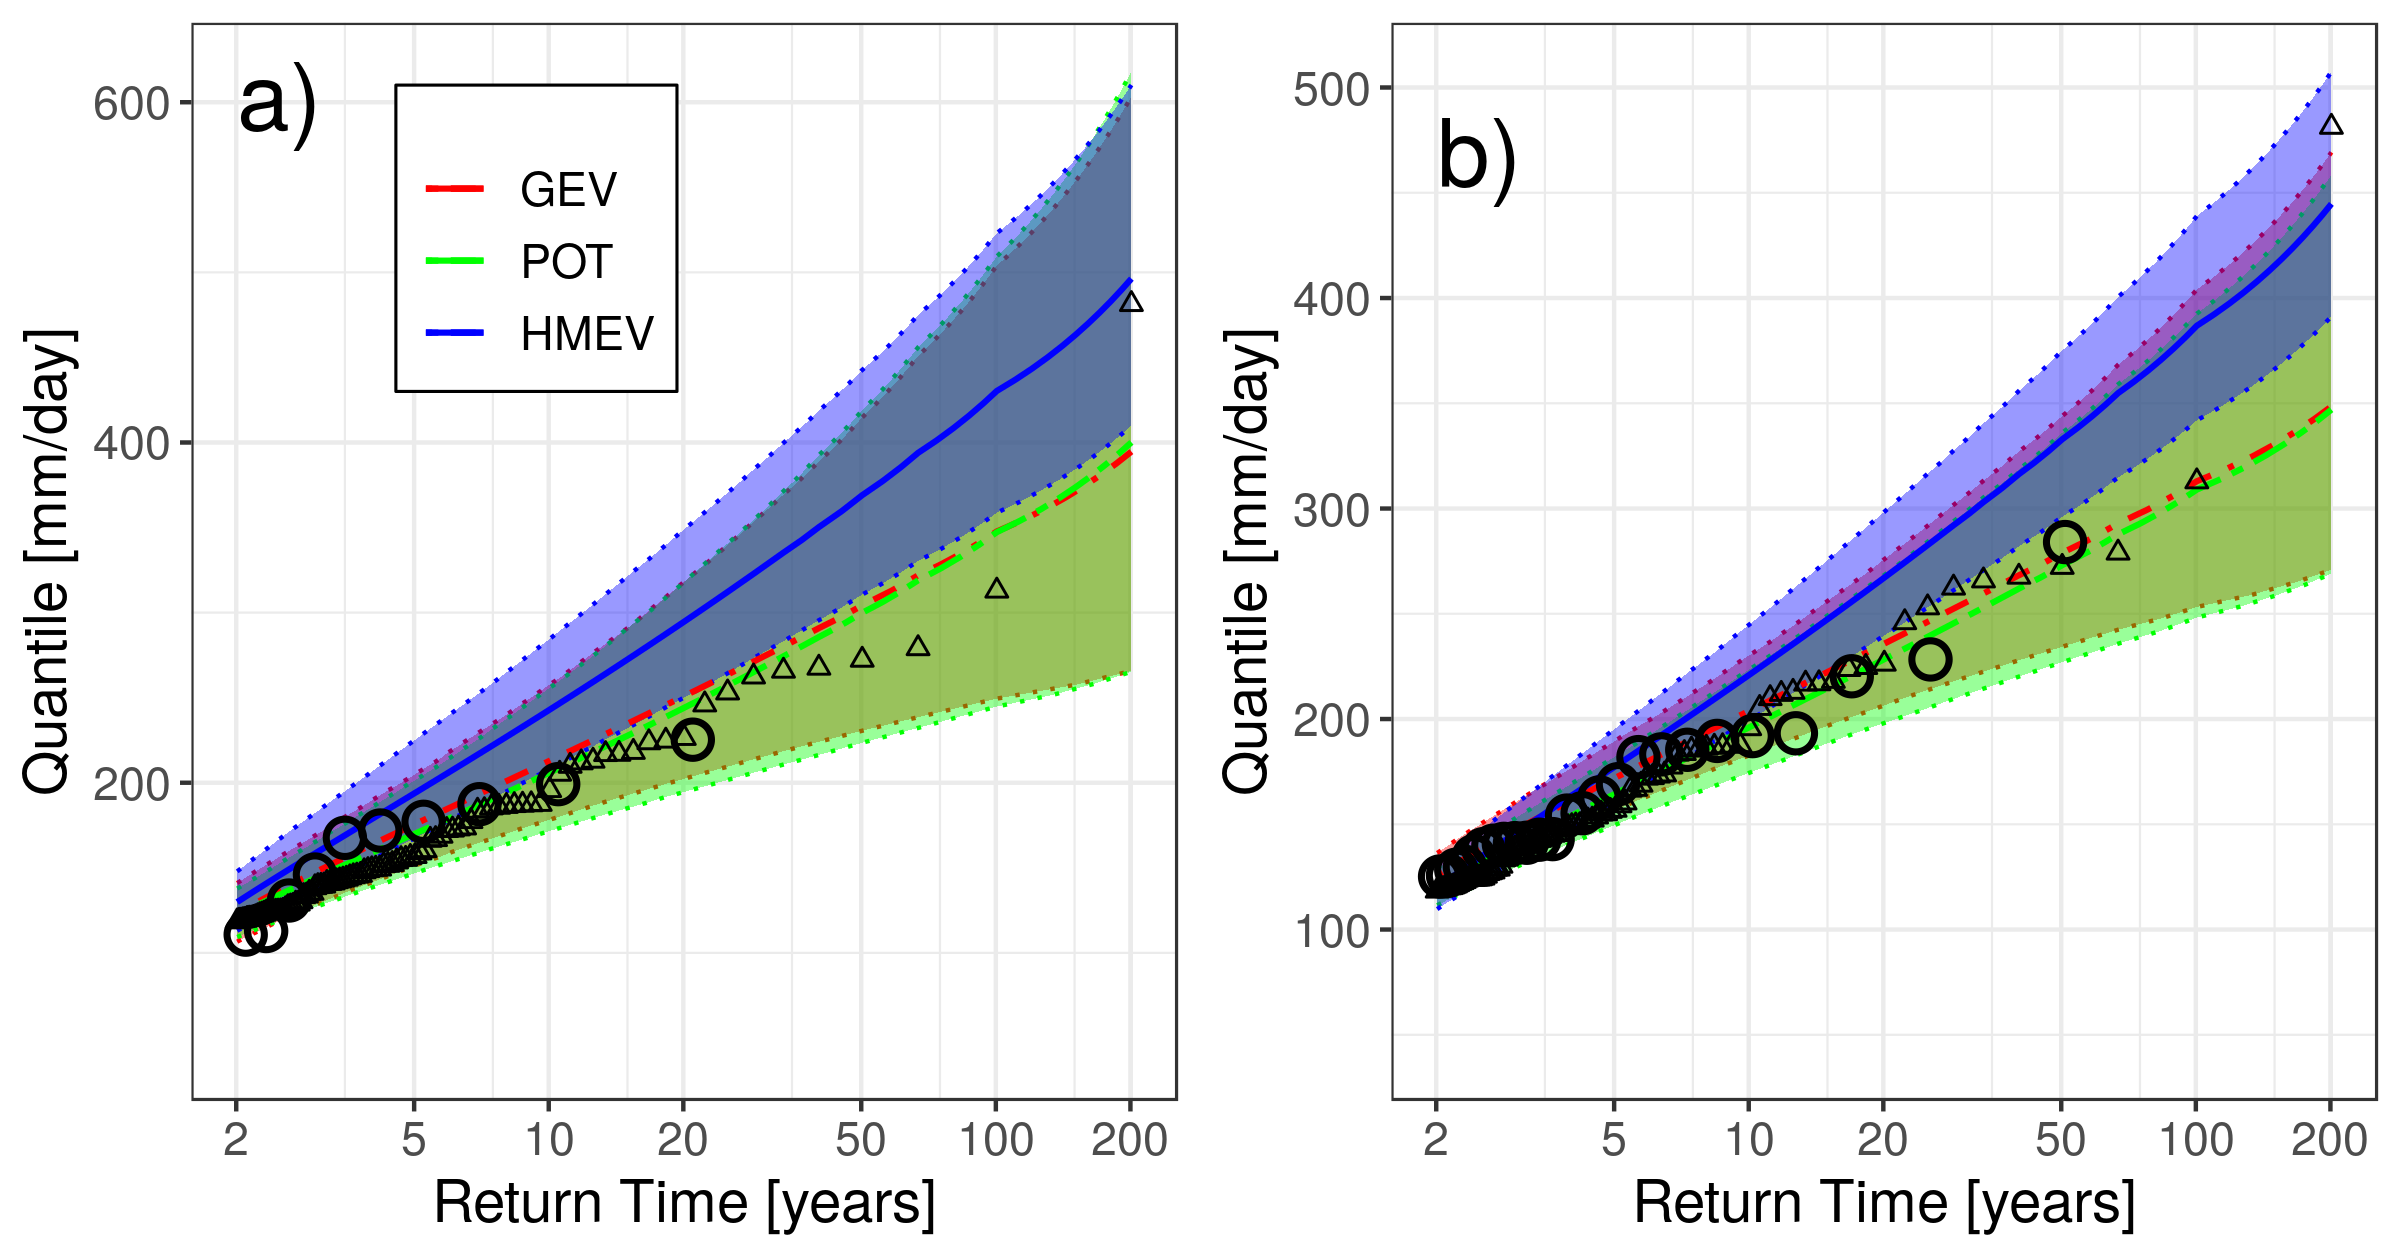
\includegraphics[width=1\linewidth]{../output/outplot/synth_examples_ss_20_50_4spec_wei} \caption{Example of fit to samples of 20 and 50 yearly blocks of data generated according to the Weibull specification.\label{fig:wei_spec}}\label{fig:wei}
\end{figure}

\begin{figure}
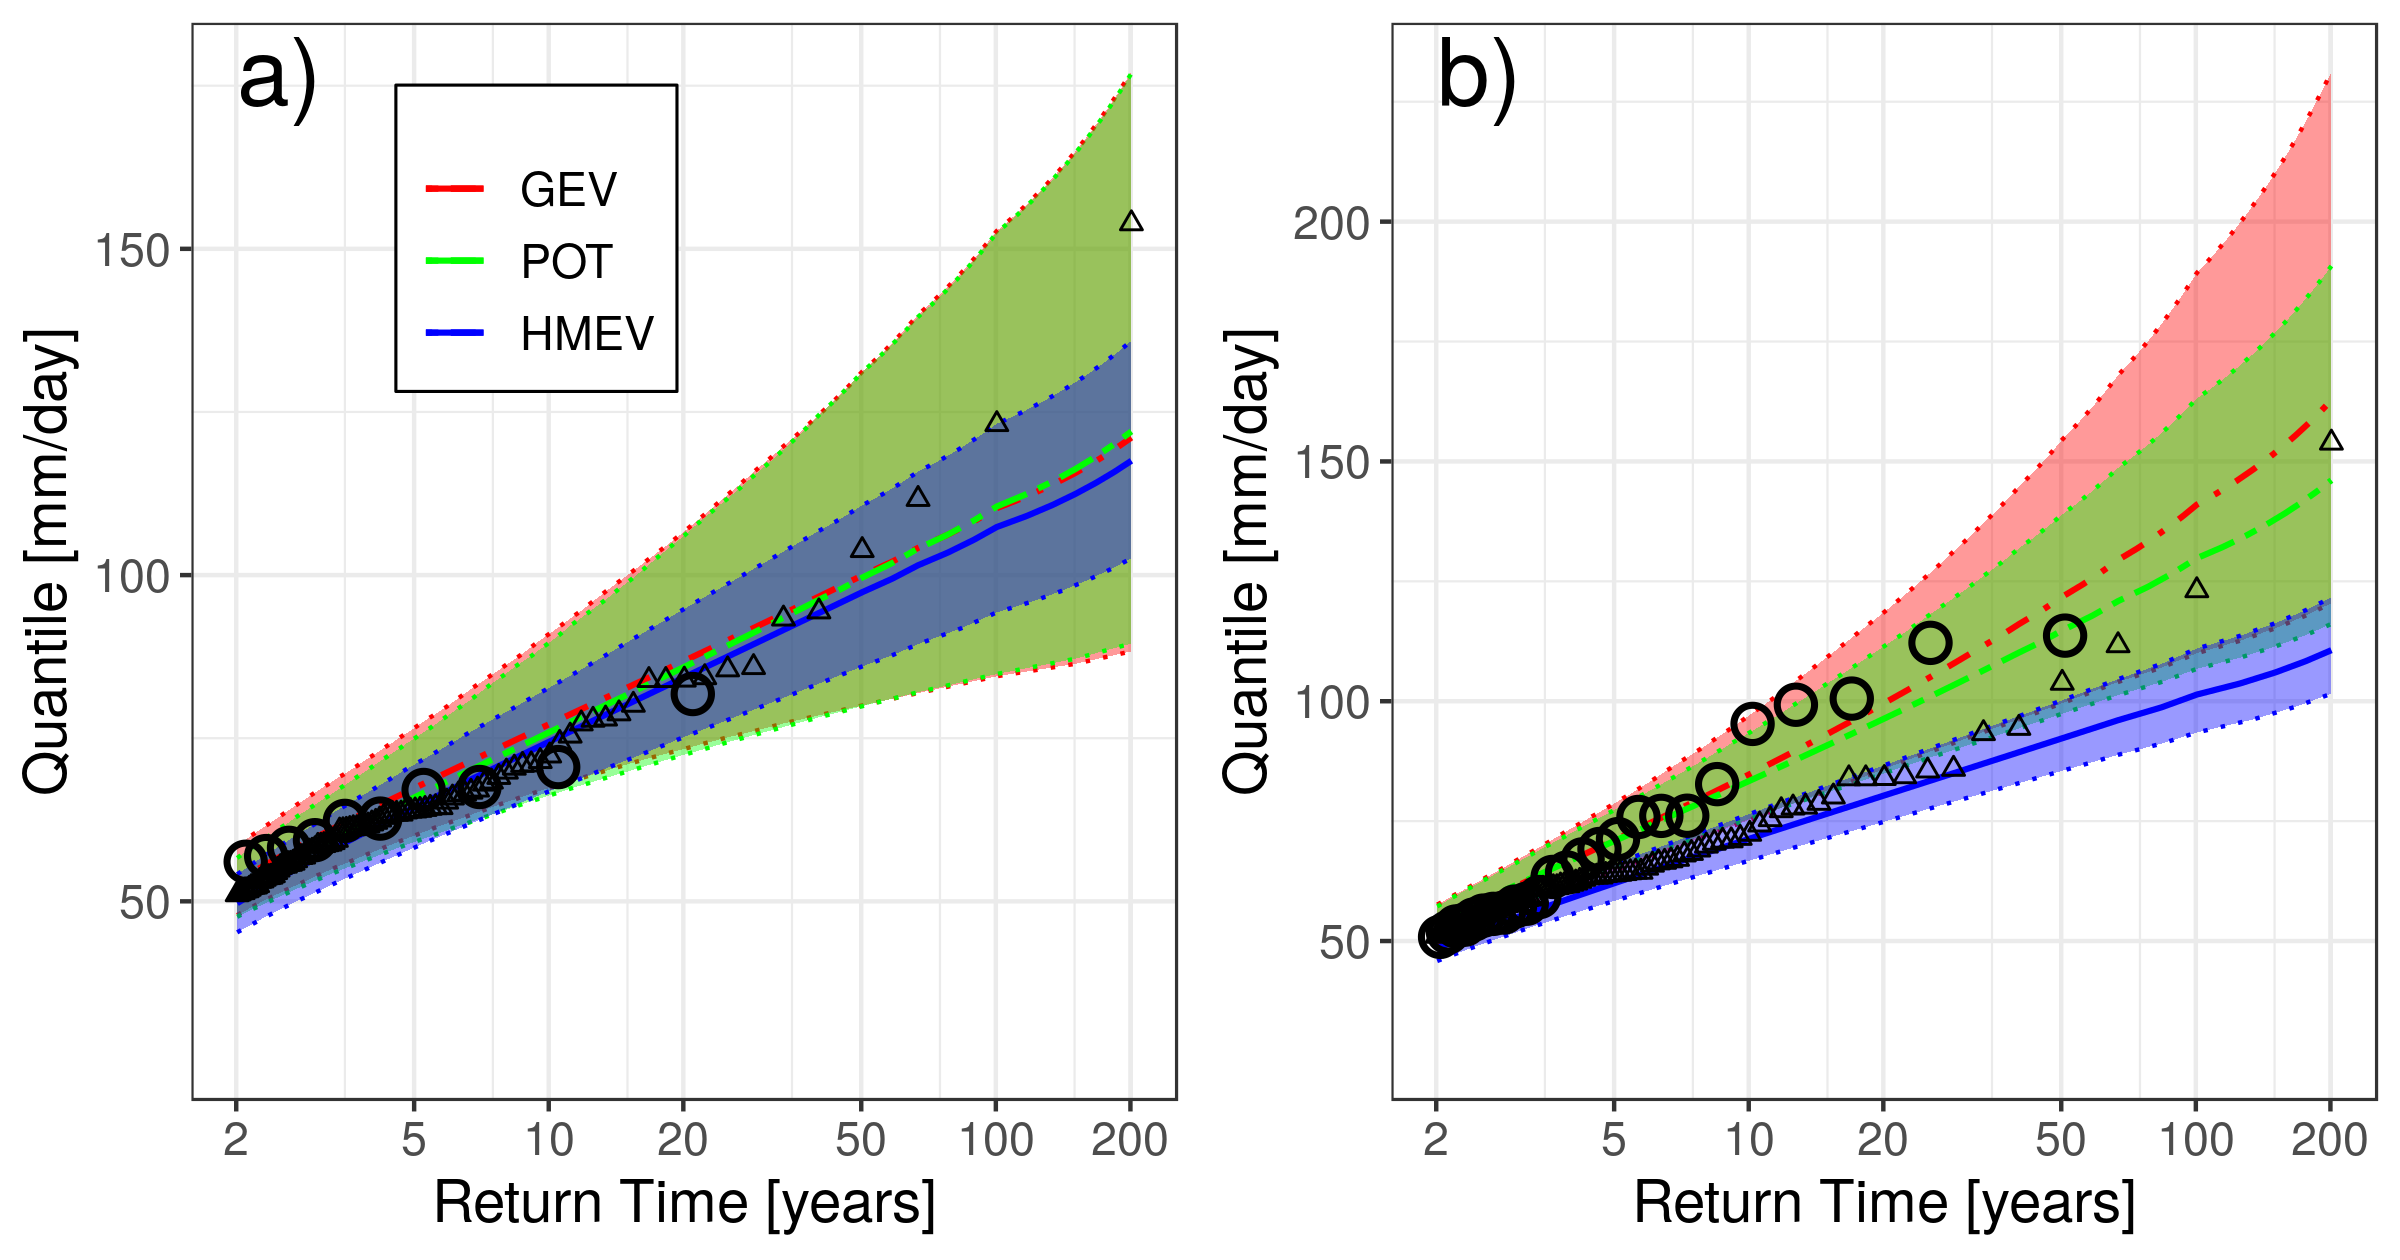
\includegraphics[width=1\linewidth]{../output/outplot/synth_examples_ss_20_50_4spec_gpd} \caption{Example of fit to samples of 20 and 50 yearly blocks of data generated according to the Generalized Pareto specification.\label{fig:gpd_spec}}\label{fig:gam}
\end{figure}

\begin{figure}
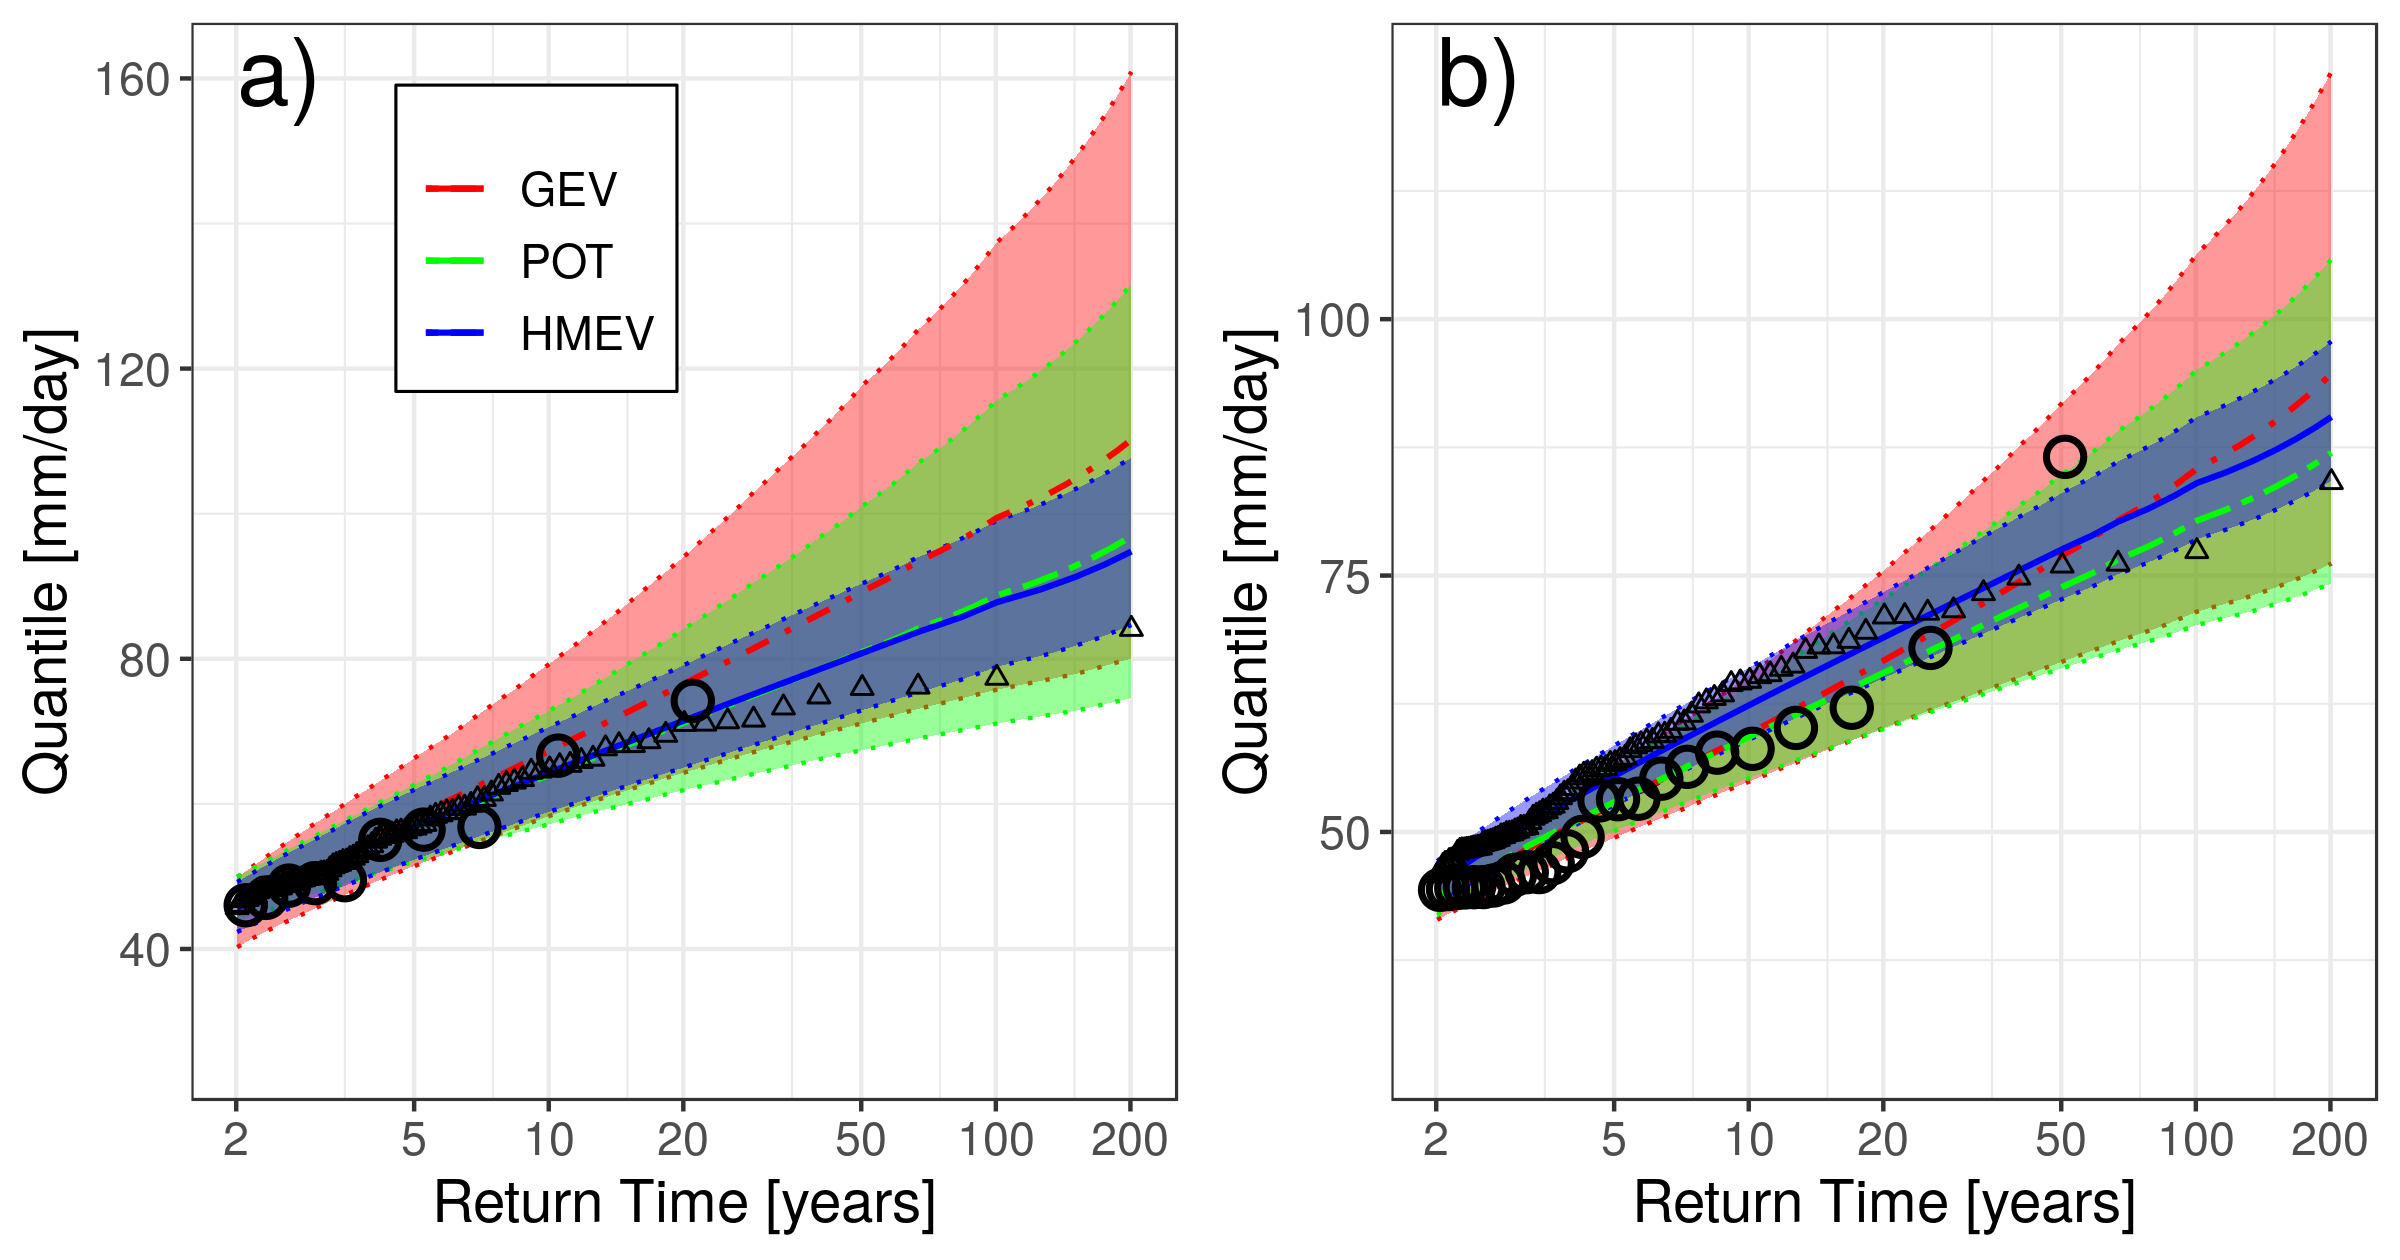
\includegraphics[width=1\linewidth]{../output/outplot/synth_examples_ss_20_50_4spec_gam} \caption{Example of fit to samples of 20 and 50 yearly blocks of data generated according to the Gamma specification.\label{fig:gam_spec}}\label{fig:gpd}
\end{figure}

\hypertarget{references}{%
\section*{References}\label{references}}
\addcontentsline{toc}{section}{References}

\hypertarget{refs}{}
\leavevmode\hypertarget{ref-coles2001introduction}{}%
Coles, Stuart. 2001. \emph{An Introduction to Statistical Modeling of
Extreme Values}. Vol. 208. Springer.

\leavevmode\hypertarget{ref-coles1996bayesian2}{}%
Coles, Stuart G, and Elwyn A Powell. 1996. ``Bayesian Methods in Extreme
Value Modelling: A Review and New Developments.'' \emph{International
Statistical Review/Revue Internationale de Statistique}. JSTOR, 119--36.

\leavevmode\hypertarget{ref-coles1996bayesian}{}%
Coles, Stuart G, and Jonathan A Tawn. 1996. ``A Bayesian Analysis of
Extreme Rainfall Data.'' \emph{Journal of the Royal Statistical Society:
Series C (Applied Statistics)} 45 (4). Wiley Online Library: 463--78.

\leavevmode\hypertarget{ref-coles2003fully}{}%
Coles, Stuart, Luis Raúl Pericchi, and Scott Sisson. 2003. ``A Fully
Probabilistic Approach to Extreme Rainfall Modeling.'' \emph{Journal of
Hydrology} 273 (1-4). Elsevier: 35--50.

\leavevmode\hypertarget{ref-davison1990models}{}%
Davison, Anthony C, and Richard L Smith. 1990. ``Models for Exceedances
over High Thresholds.'' \emph{Journal of the Royal Statistical Society.
Series B (Methodological)}. JSTOR, 393--442.

\leavevmode\hypertarget{ref-de2007extreme}{}%
De Haan, Laurens, and Ana Ferreira. 2007. \emph{Extreme Value Theory: An
Introduction}. Springer Science \& Business Media.

\leavevmode\hypertarget{ref-gelfand1994bayesian}{}%
Gelfand, Alan E, and Dipak K Dey. 1994. ``Bayesian Model Choice:
Asymptotics and Exact Calculations.'' \emph{Journal of the Royal
Statistical Society. Series B (Methodological)}. JSTOR, 501--14.

\leavevmode\hypertarget{ref-gelfand1992model}{}%
Gelfand, Alan E, Dipak K Dey, and Hong Chang. 1992. ``Model
Determination Using Predictive Distributions with Implementation via
Sampling-Based Methods.'' STANFORD UNIV CA DEPT OF STATISTICS.

\leavevmode\hypertarget{ref-gelman2013bayesian}{}%
Gelman, Andrew, John B Carlin, Hal S Stern, David B Dunson, Aki Vehtari,
and Donald B Rubin. 2013. \emph{Bayesian Data Analysis}. Chapman;
Hall/CRC.

\leavevmode\hypertarget{ref-gilleland2016extremes}{}%
Gilleland, Eric, Richard W Katz, and others. 2016. ``ExtRemes 2.0: An
Extreme Value Analysis Package in R.'' \emph{Journal of Statistical
Software} 72 (8). Foundation for Open Access Statistics: 1--39.

\leavevmode\hypertarget{ref-hosking1990moments}{}%
Hosking, Jonathan RM. 1990. ``L-Moments: Analysis and Estimation of
Distributions Using Linear Combinations of Order Statistics.''
\emph{Journal of the Royal Statistical Society: Series B
(Methodological)} 52 (1). Wiley Online Library: 105--24.

\leavevmode\hypertarget{ref-koutsoyiannis2004statistics}{}%
Koutsoyiannis, Demetris. 2004. ``Statistics of Extremes and Estimation
of Extreme Rainfall: I. Theoretical Investigation/Statistiques de
Valeurs Extrêmes et Estimation de Précipitations Extrêmes: I. Recherche
Théorique.'' \emph{Hydrological Sciences Journal} 49 (4). Taylor \&
Francis.

\leavevmode\hypertarget{ref-martins2000generalized}{}%
Martins, Eduardo S, and Jery R Stedinger. 2000. ``Generalized
Maximum-Likelihood Generalized Extreme-Value Quantile Estimators for
Hydrologic Data.'' \emph{Water Resources Research} 36 (3). Wiley Online
Library: 737--44.

\leavevmode\hypertarget{ref-stephenson2004bayesian}{}%
Stephenson, Alec, and Jonathan Tawn. 2004. ``Bayesian Inference for
Extremes: Accounting for the Three Extremal Types.'' \emph{Extremes} 7
(4). Springer: 291--307.

\leavevmode\hypertarget{ref-vehtari2017practical}{}%
Vehtari, Aki, Andrew Gelman, and Jonah Gabry. 2017. ``Practical Bayesian
Model Evaluation Using Leave-One-Out Cross-Validation and Waic.''
\emph{Statistics and Computing} 27 (5). Springer: 1413--32.

\leavevmode\hypertarget{ref-von1936distribution}{}%
Von Mises, Richard. 1936. ``La Distribution de La Plus Grande de N
Valeurs.'' \emph{Rev. Math. Union Interbalcanique} 1 (1).


\end{document}
